\section{评估}\label{sec:eval}
\SetKwInput{KwForEach}{for each}
\begin{algorithm}[h]
    \caption{One-time Remote Attestation}
    \KwIn{NULL}
    $(PK_{CSP}, SK_{CSP}) \leftarrow sgx\_ecc256\_create\_key\_pair()$\;
    Remote attestation to Intel service to verify $PK_{CSP}$'s authorization\;
    \KwForEach{data analysis task}
    \Begin{
        $SK \leftarrow Dec(SK_{CSP},Enc_{SK})$\;
        Establish a local attestation channel between EKeyMgr and EAnalyzer\;
        Use $SK$\;
    }
    \KwRet{}\;
\label{algo:attestation}
\end{algorithm}

在本节中,我们通过综合实验评估Fidelius的性能。首先,我们通过分别执行CPU密集型和I/O密集型任务来评估其时间消耗。随后,我们对Fidelius与在以太坊虚拟机(EVM)中执行分析程序的替代解决方案进行性能比较。我们的实验在一台配备Intel(R) Core(TM) i5-10400F CPU的机器上进行,该CPU拥有12个核心,频率为2.9 GHz,16 GB内存和12 MB缓存。除非另有说明,每个实验重复1,000次以计算平均值。

\subsection{CPU密集型任务}
为了评估Fidelius在CPU密集型任务上的性能,我们实现了一个具有三层和128个隐藏单元的神经网络算法,设计用于使用MNIST数据集识别手写数字~\cite{mnist}。我们报告算法的时间消耗和准确性。此外,我们在原始CPU(无SGX)上部署算法进行比较。基于Fidelius的算法与基于原始CPU的算法之间的主要差异包括:
\begin{itemize}
  \item 随机库。基于Fidelius的算法使用基于Intel SGX的随机库,而基于原始CPU的算法依赖C++随机库。
  \item 数据解密。Fidelius在启动算法前需要解密密封数据,产生额外的处理时间。相反,基于原始CPU的算法可以直接访问明文数据。
\end{itemize}
对于Fidelius和原始CPU,我们保持固定的测试集数量为1,000,同时将训练集数量从10,000逐步增加到50,000。对于每个训练集,我们分别将epoch设置为100和200来执行算法。


\begin{figure*}[h]
\centering
{
  \setlength{\tabcolsep}{0pt}
  \begin{tabular}{cccc}
\subfloat[epoch = 100]{
  \scalebox{0.39}{
  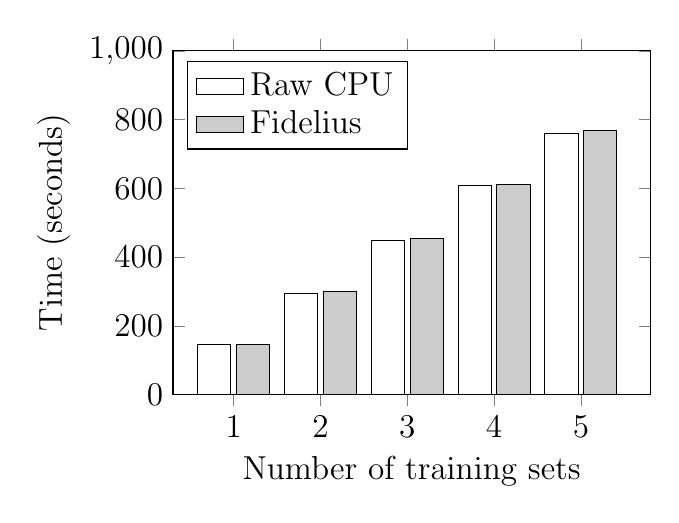
\begin{tikzpicture}
    
\begin{axis}[
  compat=newest,
  legend style={
     legend columns=1,
     font=\large,
     legend pos=north west},
  ybar,
  bar width=12pt,
  ymin=0,
  ymax=1000,
  xmin=0.3,
  xmax=5.8,
  scale only axis,
  xticklabels={\bench{\large 1}, \bench{\large 2}, \bench{\large 3},
    \bench{\large 4}, \bench{\large 5}
  },
  ylabel={Time (seconds)
  },
    xlabel=Number of training sets,
    xtick=data,
    width=0.5\textwidth,
    height=0.36\textwidth,
    every axis/.append style={font=\large,
      label style={font=\large},
      tick label style={font=\large}
    }
  ]
\addplot [area legend] coordinates{
  (1, 144.6828)
  (2, 293.267)
  (3, 447.979)
  (4, 609.104)
  (5, 758.237)
};
\addplot [fill=black!20,area legend] coordinates{
  (1, 145.0)
  (2, 298.95)
  (3, 454.3)
  (4, 612.15)
  (5, 768.33)
};
\legend{[right]{Raw CPU}, [right]{Fidelius}}
\end{axis}
\end{tikzpicture}}
} &
\subfloat[epoch = 200]{
  \scalebox{0.39}{
  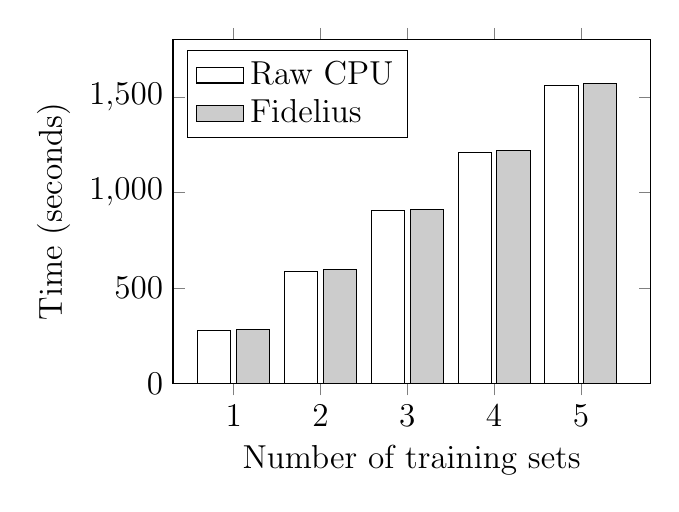
\begin{tikzpicture}
    
\begin{axis}[
  compat=newest,
  legend style={
     legend columns=1,
     font=\large,
     legend pos=north west},
  ybar,
  bar width=12pt,
  ymin=0,
  ymax=1800,
  xmin=0.3,
  xmax=5.8,
  scale only axis,
  xticklabels={\bench{\large 1}, \bench{\large 2}, \bench{\large 3},
    \bench{\large 4}, \bench{\large 5}
  },
  ylabel={Time (seconds)
  },
    xlabel=Number of training sets,
    xtick=data,
    width=0.5\textwidth,
    height=0.36\textwidth,
    every axis/.append style={font=\large,
      label style={font=\large},
      tick label style={font=\large}
    }
  ]
\addplot [area legend] coordinates{
  (1, 278.258)
  (2, 587.359)
  (3, 905.65)
  (4, 1208.9)
  (5, 1562.5)
};
\addplot [fill=black!20,area legend] coordinates{
  (1, 282)
  (2, 595.27)
  (3, 909.03)
  (4, 1219.71)
  (5, 1570)
};

\legend{[right]{Raw CPU}, [right]{Fidelius}}
\end{axis}		
\end{tikzpicture}}
} &
\subfloat[epoch = 100]{
  \scalebox{0.39}{
  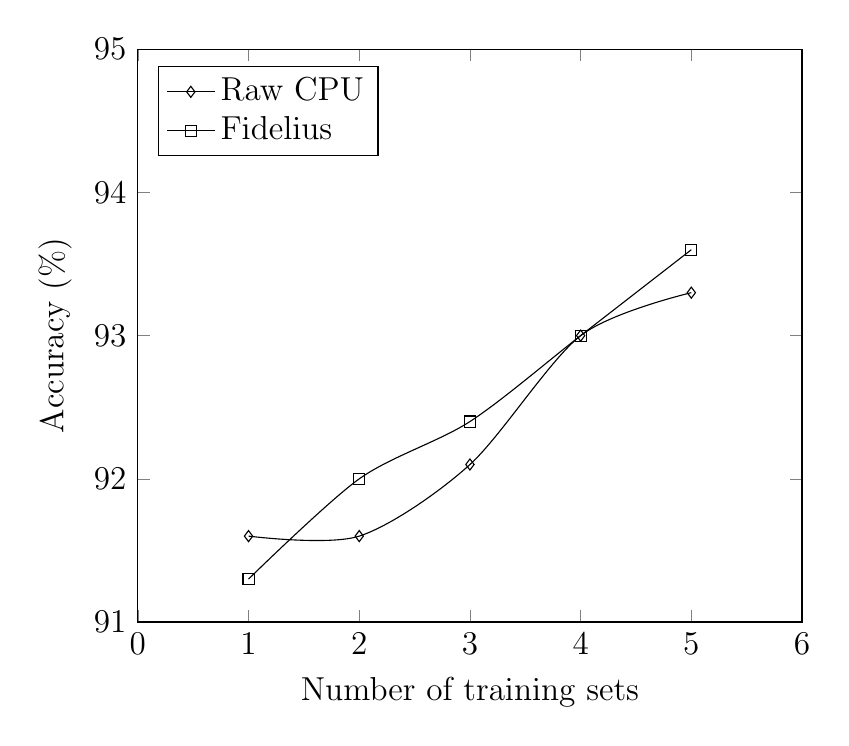
\begin{tikzpicture}
    
\large
\pgfplotsset{
    scale only axis,
    xmin=0, xmax=6,
    compat=newest,
    legend pos=north west,
}

\begin{axis}[
  %axis y line*=left,
  %scaled y ticks=base 10:2,
  %ymin=0, ymax=0.0004,
  %ymin=0, ymax=0.008,
  ymin=91, ymax=95,
  xlabel=Number of training sets,
  %width=0.4\textwidth,
  %height=0.6\textwidth,
  ylabel=Accuracy (\%),
]

\addplot[smooth,mark=diamond]
  coordinates{
    (1,91.6)
    (2,91.6)
    (3,92.1)
    (4,93.0)
    (5,93.3)
}; \label{plot_raw}

\addplot[smooth,mark=square]
  coordinates{
    (1,91.3)
    (2,92.0)
    (3,92.4)
    (4,93.0)
    (5,93.6)
  }; \label{plot_fid}



  \addlegendimage{/pgfplots/refstyle=plot_raw}\addlegendentry[right]{Raw CPU}
  \addlegendimage{/pgfplots/refstyle=plot_fid}\addlegendentry[right]{Fidelius}

\end{axis}
\end{tikzpicture}}
} &
\subfloat[epoch = 200]{
  \scalebox{0.39}{
  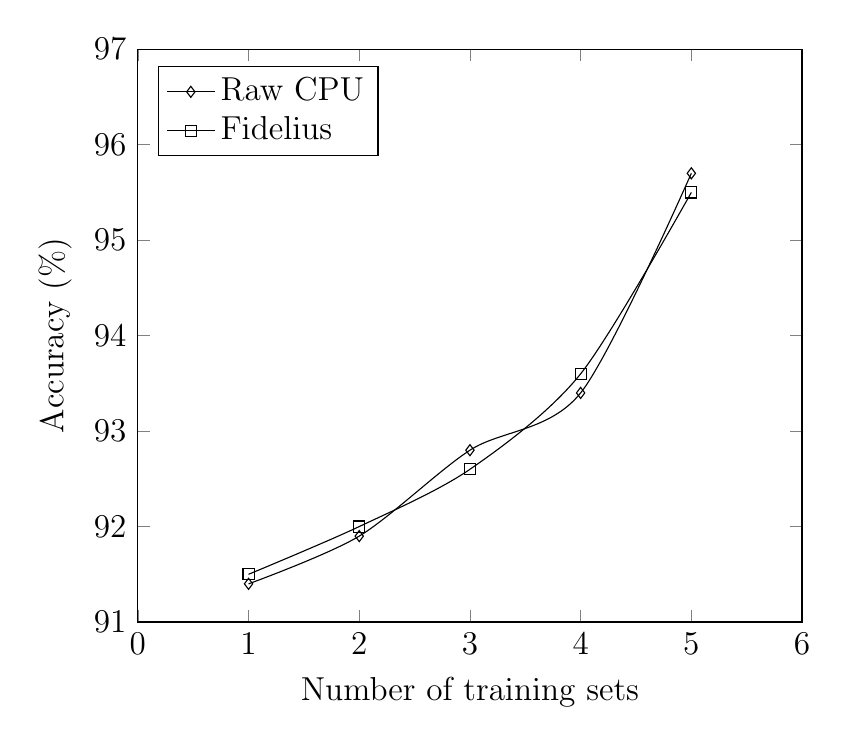
\begin{tikzpicture}
    
\large
\pgfplotsset{
    scale only axis,
    xmin=0, xmax=6,
    compat=newest,
    legend pos=north west,
}

\begin{axis}[
  %axis y line*=left,
  %scaled y ticks=base 10:2,
  %ymin=0, ymax=0.0004,
  %ymin=0, ymax=0.008,
  ymin=91, ymax=97,
  xlabel=Number of training sets,
  %width=0.4\textwidth,
  %height=0.6\textwidth,
  ylabel=Accuracy (\%),
]

\addplot[smooth,mark=diamond]
  coordinates{
    (1,91.4)
    (2,91.9)
    (3,92.8)
    (4,93.4)
    (5,95.7)
}; \label{plot_raw}

\addplot[smooth,mark=square]
  coordinates{
    (1,91.5)
    (2,92.0)
    (3,92.6)
    (4,93.6)
    (5,95.5)
  }; \label{plot_fid}



  \addlegendimage{/pgfplots/refstyle=plot_raw}\addlegendentry[right]{Raw CPU}
  \addlegendimage{/pgfplots/refstyle=plot_fid}\addlegendentry[right]{Fidelius}

\end{axis}
\end{tikzpicture}}
} \\
\end{tabular}
}
  \caption{\small Time Consumption and Accuracy of CPU-Intensive Task.}
\label{fig:cpu_intensive}
\end{figure*}


图~\ref{fig:cpu_intensive}(a)和~\ref{fig:cpu_intensive}(b)说明了在不同epoch下在Fidelius和原始CPU上运行的算法的时间消耗。随着训练集数量的增加,Fidelius和原始CPU上算法的时间消耗都呈现线性增长趋势。然而,这两种算法之间的时间消耗差异很小。具体而言,观察到Fidelius上的执行时间仅比原始CPU长2\%,主要是由于数据解密开销。

图~\ref{fig:cpu_intensive}(c)和~\ref{fig:cpu_intensive}(d)显示了在不同epoch下Fidelius和原始CPU上算法的准确性,两者都达到了超过91\%的准确性。在100个epoch时,准确性略有波动,但平台之间没有明显差异。在200个epoch时,两种算法都收敛到几乎相同的准确性。Fidelius与原始CPU相比时间消耗增加了2\%,但保持了相似的准确性水平,在CPU密集型任务中表现出可比的性能。

\subsection{I/O密集型任务}\label{subsec:io_intensive}
为了评估Fidelius在处理I/O密集型任务时的时间效率,我们在Fidelius和原始CPU平台上测试了一个在超过1 GB文件中搜索目标字符串的算法。时间消耗取决于数据加载和字符串搜索,Fidelius由于数据解密需要额外时间。考虑到Intel SGX在Fidelius中的约束,我们将数据加载块大小设置为64 KB和256 KB,并为每个块大小改变数据行数从1到128和1到256来测量时间效率。


\begin{figure}[h]
  \centering
{
\begin{tabular}{cc}
      \subfloat[Data block size = 64 KBytes]{
        \scalebox{0.39}{
          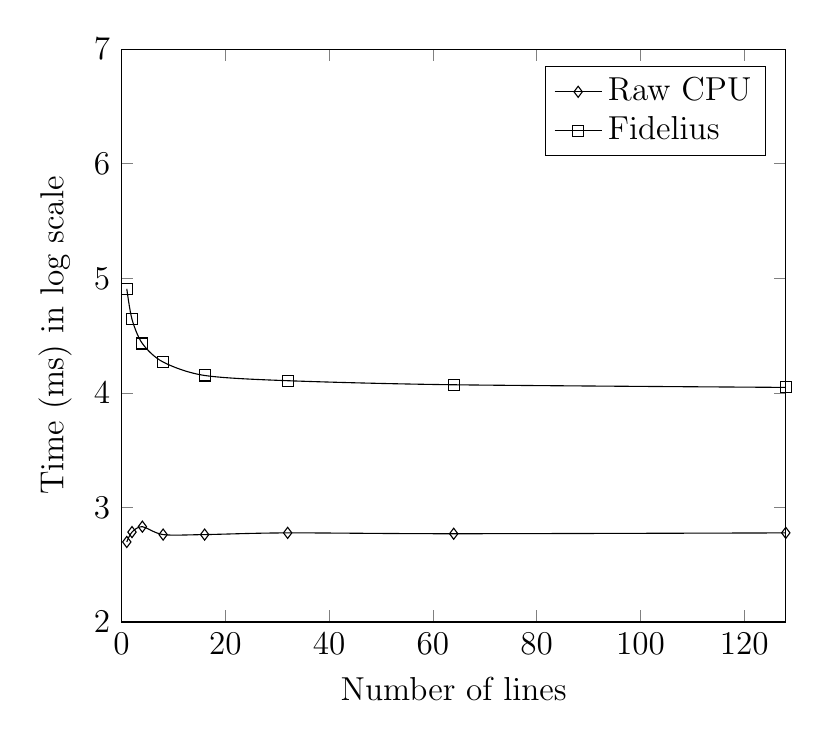
\begin{tikzpicture}
            
\large
\pgfplotsset{
    scale only axis,
    xmin=0, xmax=128,
    compat=newest,
    legend pos=north east,
}

\begin{axis}[
  %axis y line*=left,
  %scaled y ticks=base 10:2,
  %ymin=0, ymax=0.0004,
  %ymin=0, ymax=0.008,
  ymin=2, ymax=7,
  xlabel=Number of lines,
  %width=0.4\textwidth,
  %height=0.6\textwidth,
  ylabel=Time (ms) in log scale,
]

\addplot[smooth,mark=diamond]
  coordinates{
    (1,2.6990) %log10(500)
    (2,2.7853) %log10(610)
    (4,2.8325) %log10(680)
    (8,2.7634) %log10(580)
    (16,2.7634) %log10(580)
    (32,2.7782) %log10(600)
    (64,2.7709) %log10(590)
    (128,2.7782) %log10(600)
}; \label{plot_raw}

\addplot[smooth,mark=square]
  coordinates{
    (1,4.9085) %log10(81000)
    (2,4.6435) %log10(44000)
    (4,4.4314) %log10(27000)
    (8,4.2695) %log10(18600)
    (16,4.1523) %log10(14200)
    (32,4.1065) %log10(12780)
    (64,4.0711) %log10(11780)
    (128,4.0481) %log10(11170)
  }; \label{plot_fid}



  \addlegendimage{/pgfplots/refstyle=plot_raw}\addlegendentry[right]{Raw CPU}
  \addlegendimage{/pgfplots/refstyle=plot_fid}\addlegendentry[right]{Fidelius}

\end{axis}
          \end{tikzpicture}
        }
      } &
      \subfloat[Data block size = 256 KBytes]{
        \scalebox{0.39}{
          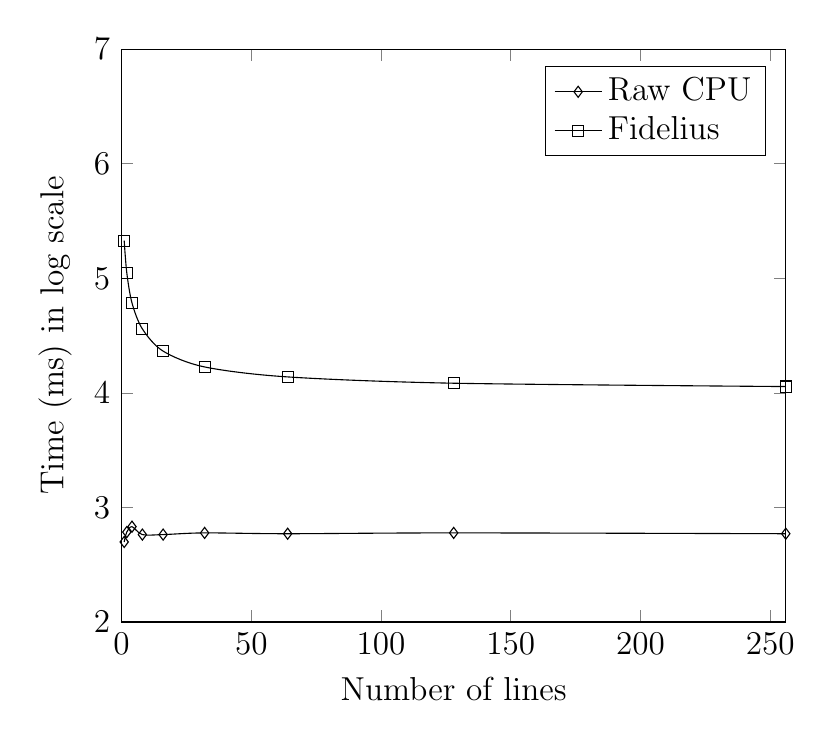
\begin{tikzpicture}
            
\large
\pgfplotsset{
    scale only axis,
    xmin=0, xmax=256,
    compat=newest,
    legend pos=north east,
}

\begin{axis}[
  %axis y line*=left,
  %scaled y ticks=base 10:2,
  %ymin=0, ymax=0.0004,
  %ymin=0, ymax=0.008,
  ymin=2, ymax=7,
  xlabel=Number of lines,
  %width=0.4\textwidth,
  %height=0.6\textwidth,
  ylabel=Time (ms) in log scale,
]
1	0.5	    213
2	0.61	111.78
4	0.68	61.04
8	0.58	36.2
16	0.58	23.16
32	0.6	    16.85
64	0.59	13.79
128	0.6	    12.15
256	0.59	11.36
\addplot[smooth,mark=diamond]
  coordinates{
    (1,2.6990) %log10(500)
    (2,2.7853) %log10(610)
    (4,2.8325) %log10(680)
    (8,2.7634) %log10(580)
    (16,2.7634) %log10(580)
    (32,2.7782) %log10(600)
    (64,2.7709) %log10(590)
    (128,2.7782) %log10(600)
    (256, 2.7709) %log10(590)
}; \label{plot_raw}

\addplot[smooth,mark=square]
  coordinates{
    (1,5.3284) %log10(213000)
    (2,5.0484) %log10(111780)
    (4,4.7856) %log10(61040)
    (8,4.5587) %log10(36200)
    (16,4.3647) %log10(23160)
    (32,4.2266) %log10(16850)
    (64,4.1396) %log10(13790)
    (128,4.0846) %log10(12150)
    (256,4.0554) %log10(11360)
  }; \label{plot_fid}



  \addlegendimage{/pgfplots/refstyle=plot_raw}\addlegendentry[right]{Raw CPU}
  \addlegendimage{/pgfplots/refstyle=plot_fid}\addlegendentry[right]{Fidelius}

\end{axis}
          \end{tikzpicture}
        }
      }    \\
\end{tabular}
  }
  \caption{\small Time Consumption of I/O-Intensive Task.}
  \label{fig:io_intensive}
\end{figure}

图~\ref{fig:io_intensive}显示了Fidelius与原始CPU在不同数据块大小下的时间效率比较。随着读取行数的增加,Fidelius的时间消耗显著减少。例如,在64 KB块大小时,Fidelius的时间从81秒(1行)下降到11秒(128行)。类似地,在256 KB块大小时,从213秒(1行)减少到10秒(256行)。将块大小增加到256 KB进一步优化了Fidelius的性能。尽管有所改进,Fidelius与原始CPU之间的时间消耗仍存在差距,主要是由于I/O密集型任务中的解密过程。

\subsection{性能比较}\label{subsec:evm_cmp}
在本节中,我们将Fidelius与SDTE~\cite{dai2019sdte}的性能进行比较,SDTE使用\textit{k}-最近邻(\textit{k}-NN)算法作为以太坊智能合约在以太坊虚拟机(EVM)上执行机器学习任务。我们在Fidelius和原始CPU上实现\textit{k}-NN算法来评估每个解决方案的时间消耗,使用来自Kaggle的Titanic数据集作为输入。

为了评估\textit{k}-NN算法在以太坊虚拟机(EVM)上的执行时间,我们在Ganache(个人以太坊区块链)上部署了\textit{k}-NN智能合约。报告的EVM上\textit{k}-NN的时间消耗仅关注执行时间,不包括交易广播或提交所花费的时间。我们还排除了将Titanic数据集上传到区块链所需的时间,因为\textit{k}-NN合约使用链上数据。由于EVM的内存限制,\textit{k}-NN算法无法处理超过60个测试集,因此我们将测试集限制在10-60个,同时保持训练集为100个。


\begin{figure}[h]
\centering
\scalebox{.8}
{
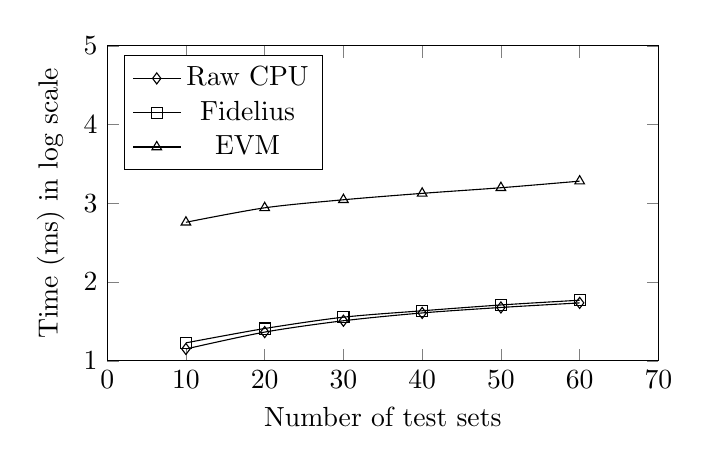
\begin{tikzpicture}
    
\pgfplotsset{
    scale only axis,
    xmin=0, xmax=70,
    ymin=1, ymax=5,
    compat=newest,
    legend pos=north west,
}

\begin{axis}[
  %axis y line*=left,
  %scaled y ticks=base 10:2,
  x=0.1cm,
  y=1cm,
  xlabel=Number of test sets,
  %width=0.4\textwidth,
  %height=0.6\textwidth,
  ylabel=Time (ms) in log scale,
]

\addplot[smooth,mark=diamond]
  coordinates{
    (10,1.1501) %log10(14.13)
    (20,1.3642) %log10(23.13)
    (30,1.5083) %log10(32.23)
    (40,1.6076) %log10(40.51)
    (50,1.6771) %log10(47.54)
    (60,1.7350) %log10(54.32)
}; \addlegendentry{Raw CPU}

\addplot[smooth,mark=square]
  coordinates{
    (10,1.2276) %log10(16.89)
    (20,1.4096) %log10(25.68)
    (30,1.5535) %log10(35.77)
    (40,1.6350) %log10(43.15)
    (50,1.7088) %log10(51.14)
    (60,1.7693) %log10(58.79)
  }; \addlegendentry{Fidelius}

\addplot[smooth,mark=triangle]
  coordinates{
    (10,2.7589) %log10(574)
    (20,2.9425) %log10(876)
    (30,3.0449) %log10(1109)
    (40,3.1261) %log10(1337)
    (50,3.1976) %log10(1576)
    (60,3.2813) %log10(1911)
  }; \addlegendentry{EVM}

\end{axis}
\end{tikzpicture}
}
  

  \caption{\small Time Consumption on Raw CPU, Fidelius and EVM.}
\label{fig:knn_cmp}
\end{figure}

图~\ref{fig:knn_cmp}显示了\textit{k}-NN算法在原始CPU、Fidelius和以太坊虚拟机(EVM)上的时间消耗,后者比其他的大约长30倍。此外,由于内存约束,EVM执行在测试超过60个集时经常失败,突出了在EVM上运行具有大数据集的复杂机器学习算法的困难,正如之前关于以太坊内存限制的研究所指出的那样~\cite{dinh2017blockbench}。相比之下,Fidelius为复杂的机器学习任务提供了更可靠和稳定的环境。 